% Template created by Karol Kozioł (www.karol-koziol.net) for ShareLaTeX

\documentclass[a4paper,portuguese,9pt,final]{extarticle}
\usepackage[utf8]{inputenc}

\usepackage[T1]{fontenc}
\usepackage{verbatim}
\usepackage{graphicx}
\usepackage{xcolor}
\usepackage{pgf,tikz}

\usepackage{enumitem}
\usepackage{flexisym}

\usetikzlibrary{shapes, calc, shapes, arrows, babel}

\usepackage{amsmath,amssymb,amsthm,textcomp}
\everymath{\displaystyle}
\usepackage{mathrsfs}
\usepackage{times}
\renewcommand\familydefault{\sfdefault}
\usepackage{tgheros}
% \usepackage[defaultmono,scale=0.85]{droidmono}

\usepackage{multicol}
\setlength{\columnseprule}{0pt}
\setlength{\columnsep}{20.0pt}

\usepackage[utf8]{inputenc}
\usepackage[portuguese]{babel}
\usepackage{eurosym}

\usepackage{graphicx}
\graphicspath{{./img/}}
\usepackage{svg}

\usepackage{hyperref}

\usepackage{geometry}
\geometry{
a4paper,
total={210mm,297mm},
left=10mm,right=10mm,top=10mm,bottom=15mm}

\linespread{1.3}

\newcommand{\samedir}{\mathbin{\!/\mkern-5mu/\!}}

% custom title
\makeatletter
\renewcommand*{\maketitle}{%
\noindent
\begin{minipage}{0.6\textwidth}
\begin{tikzpicture}
\node[rectangle,rounded corners=6pt,inner sep=10pt,fill=blue!50!black,text width= 0.95\textwidth] {\color{white}\Huge \@title};
\end{tikzpicture}
\end{minipage}
\hfill
\begin{minipage}{0.35\textwidth}
\begin{tikzpicture}
\node[rectangle,rounded corners=3pt,inner sep=10pt,draw=blue!50!black,text width= 0.95\textwidth] {\begin{tabular}{cc} \multirow{2}{1cm}{
\includegraphics[width=0.15\columnwidth]{brasao}}& \@author \\ & \ies \end{tabular}};
\end{tikzpicture}
\end{minipage}
\bigskip\bigskip
}%
\makeatother

% custom section
\usepackage[explicit]{titlesec}
\newcommand*\sectionlabel{}
\titleformat{\section}
  {\gdef\sectionlabel{}
   \normalfont\sffamily\Large\bfseries\scshape}
  {\gdef\sectionlabel{\thesection\ }}{0pt}
  {
\noindent
\begin{tikzpicture}
\node[rectangle,rounded corners=3pt,inner sep=4pt,fill=blue!50!black,text width= 0.95\columnwidth] {\color{white}\sectionlabel#1};
\end{tikzpicture}
  }
\titlespacing*{\section}{0pt}{15pt}{10pt}


% custom footer
\usepackage{fancyhdr}
\makeatletter
\pagestyle{fancy}
\fancyhead{}
\fancyfoot[C]{\footnotesize \@author \  \ies}
\renewcommand{\headrulewidth}{0pt}
\renewcommand{\footrulewidth}{0pt}
\makeatother
\usepackage{multirow} % para las tablas

\title{Séries de Fourier}
\author{Programa de Pós-Graduação}
\newcommand{\ies}{em Engenharia Civil}

\newtheorem{theorem}{Teorema}[section]
\newtheorem*{definition}{Definição}
\newtheorem*{remark}{Observação}
\newtheorem{corollary}{Corolário}[section]
\newtheorem{lema}{Lema}[section]
\newtheorem{example}{Exemplo}[section]


\providecommand{\sin}{} \renewcommand{\sin}{sen}


\begin{document}
\maketitle

\begin{multicols*}{2}



    \section{Bases de Espaços de Dimensão Infinita}

        \subsection{Produto Interno e Norma}

            \begin{definition}

                Produto Interno ou Escalar: um produto interno ou escalar num espaço vetorial $ V $ é o mapa (bilinear) definido por:

                (  $ \cdot $  ,  $ \cdot $  ) : $ V $ x $ V \to \mathbb{R} $ que possui, para todos $ x, y $ e $  z  \in  V  $ e $ \alpha \in  \mathbb{R} $, as seguintes propriedades:


                \begin{description}
                    \item[(i)] $ (x,y) = (y,x) ;$
                    \item[(ii)] $ (\alpha x,y) =  \alpha (x,y) ;$
                    \item[(iii)] $(x+y,z) = (x,z) + (y,z);$
                    \item[(iv)] $ (x,x) > 0 \iff x \neq 0 .$
                \end{description}

            \end{definition}

            \begin{example}
                A integral $$ \int_{a}^{b} f(x)g(x) dx$$ é um produto interno do  espaço $ C^{0}[a,b] $. 
            \end{example}
            Consequências da definição de produto interno:

            \begin{description}
                \item[(i)] $(x,y+z) = (x,y) + (x,z);$
                \item[(ii)] $ (x,\alpha y) = \alpha (x,y) ;$
                \item[(iii)] $ (x,0) = 0 = (0,x) ;$
                \item[(iv)] Se $ (x,z) = (y,z) $ para todo $ z \in V $, então $ x = y. $
            \end{description}
            
            \begin{definition}

            Norma: A norma de $ x \in V $ ($ V $ é um espaço vetorial dotado de produto interno) é definido por $ ||x||=(x,x)^{\frac{1}{2}} $. 


            \end{definition}

            \begin{example}
                Para um espaço como o $ \mathbb{R}^{n}(x=[x_{1},x_{2},...,x_{n}]^{T}) $ temos que $ ||x||=\sqrt{|x_{1}|^{2}+|x_{2}|^{2}+...+|x_{n}|^{2}} $. 
            \end{example}


            \begin{example}
                Para o espaço $ C^{0}[a,b] $ do exemplo 1.1 temos $$ ||f|| = \{\int_{a}^{b} |f(x)|^{2}dx\}^{\frac{1}{2}} $$. \\
            \end{example}


            \textit{OBS:} Nos Teoremas e resultados a serem enunciados a seguir, sempre que houver menção ao espaço $ V $ entenda que estamos nos referindo a um espaço vetorial com produto interno e norma associada a este produto interno. 

            \begin{theorem}
                Para quaisquer $ x $ e $ y \in V $ e $ \alpha \in \mathbb{R} $, vale:

                \begin{description}
                    \item[(i)] $ ||x||\geq 0 ; ||x|| = 0$ se e somente se $ x=0; $ 
                    \item[(ii)] $ ||\alpha x|| = |\alpha| ||x||; $
                    \item[(iii)] $ ||x+y|| \leq ||x|| + ||y|| $
                \end{description} 
            \end{theorem}

            \begin{theorem}
                Desigualdade de Cauchy-Schwarz: para $ x $ e $ y \in V $ vale:

                $$ |(x,y)|\leq ||x||\cdot ||y||$$ \

            \end{theorem}

            \begin{theorem}
                Lei do Paralelogramo: para vetores $ x, y \in V $ tem-se:

                $$ ||x+y||^{2} + ||x-y||^{2} =  2 ||x||^{2} + 2 ||y||^{2} $$ \\
            \end{theorem}

            Para um espaço vetorial $ V $ de dimensão finita ($ dim(V)=n $) e com uma base ortonormal (ortogonal e normalizada) $ e_{1},...,e_{n} $, podemos escrever para todo $ x \in V $:

            \begin{equation}
            x=(x,e_{1})e_{1}+...+(x,e_{n})e_{n}
            \label{71}
            \end{equation}

            Esse conceito pode ser estendido para os casos em que $ dim(V)=\infty $; nestes casos, podemos escrever o lado direito de (\ref{71}) como:

            \begin{equation}
            \sum_{i=1}^{\infty} (x,e_{i})e_{i}
            \label{72}
            \end{equation}


            É claro que (\ref{72}) só faz sentido para espaços de dimensão infinita com bases contáveis. Quando essa série converge, dizemos que ela converge na média para $ x $, logo podemos dizer que:

            $$\displaystyle  x = \sum_{i=1}^{\infty} (x,e_{i})e_{i}  $$
            e dizemos que $ (x,e_{i}) $ são os coeficientes generalizados de Fourier de $ x $ com respeito à base ortonormal $ e_{1}, e_{2},... $. 
            \

            \begin{theorem}

                Seja $$\displaystyle \sum_{i=1}^{\infty}a_{i}e_{i} $$ uma série infinita que converge em média para $ x $, isto é, $$\displaystyle x=\sum_{i=1}^{\infty}a_{i}e_{i},$$ então $$ a_{i}=(x,e_{i}) $$ para todo $ i=1,2,... $. \\ \\ 

            \end{theorem}

            \begin{definition}
                Polinômio Trigonométrico: definiremos como polinômio trigonométrico de grau $ 2n+1 $ a seguinte expressão:

                \begin{equation}
                    \begin{split}
                        \displaystyle f(x) = \frac{a_{0}}{2} + a_{1}\cos(x) + a_{2}\cos(2x) + ... + a_{n}\cos(nx) +\\
                            b_{1}sen(x) + b_{2}sen(2x) + ... + b_{n}sen(nx),
                    \end{split}
                \end{equation}
                onde $ a_{0}, a_{1},...,a_{n} $ e $ b_{1}, b_{2},...,b_{n} $ são números reais e $ a_{n}\neq0 $ e/ou $ b_{n}\neq0 $. Seja $ \mathcal{F}_{n} $ o conjunto de todos os polinômios de grau $ \leq 2n+1 $ (juntamente com o polinômio 0). O espaço $ \mathcal{F}_{n} $ é um espaço vetorial com produto interno dado por:


                $$  (f,g)=\int_{-\pi}^{\pi} f(x)g(x)dx   $$ 
            \end{definition}



            O conjunto de funções $ 1, cos(x), sen(x), ... , cos(nx), sen(nx) $, é um conjunto ortogonal do espaço $ \mathcal{F}_{n} $, uma vez que para $ m $ e $ n $ inteiros:

            $$ \int_{-\pi}^{\pi} sen(mx)sen(nx)dx=0 \ ,\ se \ m\neq n, $$
            $$ \int_{-\pi}^{\pi} sen(mx)cos(nx)dx=0 \ ,$$
            $$ \int_{-\pi}^{\pi} cos(mx)cos(nx)dx=0 \ ,\ se \ m\neq n .$$ 


            Para normalizar o conjunto de funções ortogonais de $ \mathcal{F}_{n} $, podemos calcular:

            $$ \int_{-\pi}^{\pi}(1)dx=2\pi $$ e $$\ \int_{-\pi}^{\pi}sen^{2}(mx)dx=\int_{-\pi}^{\pi}cos^{2}(mx)dx=\pi \ se \ m>0.   $$



            Então as funções $ \displaystyle\frac{1}{\sqrt{2\pi}}, \frac{cos(x)}{\sqrt{\pi}}, ... , \frac{cos(nx)}{\sqrt{\pi}}, \frac{sen(x)}{\sqrt{\pi}}, ... , \frac{sen(nx)}{\sqrt{\pi}} $ são um conjunto ortonormal de $ \mathcal{F}_{n} $.

            \smallskip

            Por extensão, o conjunto infinito $$1, cos(x), sen(x), ... , cos(nx), sen(nx), ...$$ é um conjunto ortogonal em $ C^{0}[-\pi,\pi] $, além disso, esse conjunto é LI, logo esse conjunto é uma base para $ C^{0}[-\pi,\pi]. $ \\


        \subsection{Desigualdade de Bessel e Identidade de Parseval}

                
            \begin{theorem}

                Sejam $ e_{1}, e_{2}, ... $, vetores ortonormais de um espaço com produto interno e de dimensão infinita $ V $. Seja $ x \in V $, então vale a seguinte desigualdade:

                $$  \sum_{i=1}^{\infty} (x,e_{i})^{2} \leq ||x||^{2} \ \ \mbox{   (Desigualdade de Bessel).}$$


                Ainda, $ e_{1}, e_{2}, ... $, formam uma base de $V$ se e somente se:
                $$  \sum_{i=1}^{\infty} (x,e_{i})^{2} = ||x||^{2} \ \ \mbox{ (Identidade de  Parseval).}$$ 
            \end{theorem}


            A desigualdade de Bessel nos fornece uma estimativa para os coeficientes generalizados de Fourier de $x$ em relação à base $ e_{1}, e_{2}, ... $.  \\ \\

            \begin{corollary}
                Se $ e_{1}, e_{2}, ... $, for um conjunto ortonormal de um espaço $V$ de dimensão infinita dotado de produto interno, então

                $$  \lim\limits_{i\to\infty} (x,e_{i})=0  $$
                para todo $ x \in V $, ou seja, os coeficientes de Fourier de $x$ tendem a zero para $i\to\infty$ para qualquer conjunto ortonormal de $V$. \\
            \end{corollary}


            \textit{OBS:} Em muitas aplicações, prefere-se trabalhar com um conjunto ortogonal ao invés de um conjunto ortonormal. Assim sendo, a expressão em série de $x$ fica:

            $$  x=\sum_{i=1}^{\infty} \frac{(x,e_{i})}{||e_{i}||^{2}} e_{i} \ ,  $$ onde $ \displaystyle \frac{(x,e_{i})}{||e_{i}||^{2}}, i=1,2,... $, são os coeficientes generalizados de Fourier em relação ao conjunto $ e_{1}, e_{2}, ... $. \\


    \section{O Espaço de Funções Contínuas por Partes}

        \textbf{\textit{Definição}}(Função contínua por partes): uma função real $f$ é contínua por partes no intervalo $[a,b]$ se:


        \begin{description}
            \item[(i)] $f$ é definida e contínua em todos os pontos, exceto num conjunto finito de pontos de $[a,b]$;
            \item[(ii)] os limites $ f(x_{0}^{+}) = \displaystyle\lim\limits_{h\to0^{+}} f(x_{0}+h) \ e \  f(x_{0}^{-}) = \lim\limits_{h\to0^{-}} f(x_{0}-h) $ existem em cada ponto $x_{0}$ em $[a,b]$. 

            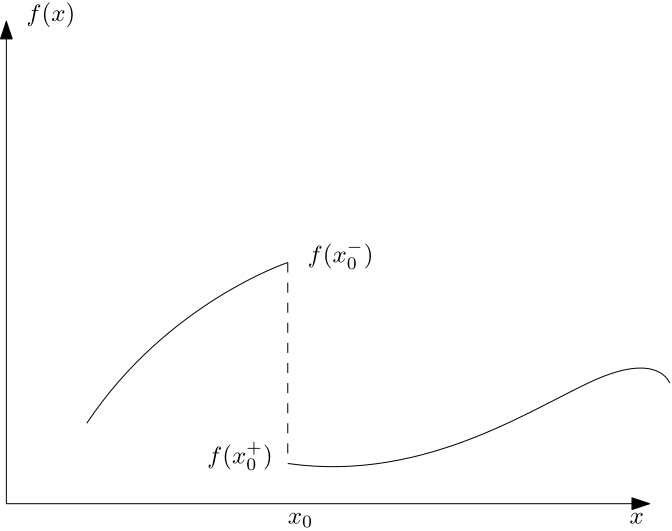
\includegraphics[width=0.4\textwidth]{funcao_cp}

            Quando um ponto $x$ é um ponto de continuidade $\displaystyle f(x_{0}^{+}) = f(x_{0}^{-}) = f(x_{0}) $. Além disso, se houver descontinuidade, ela deve ser finita.
        \end{description}


        Se $f(x)$ é contínua por partes em $[a,b]$, então $f(x)$ é integrável a Riemann e o valor dessa integração no intervalo $[a,b]$ independe dos valores que $f(x)$ assume nos pontos de descontinuidade. E em particular, podemos definir uma classe de equivalência: se $ f(x) $ e $ g(x) $ são idênticas, exceto em pontos de descontinuidade, então $\displaystyle \int_{a}^{b} f(x)dx=\int_{a}^{b} g(x)dx $. 


        Se $f(x)$ e $g(x)$ são contínuas por partes em $[a,b]$, então o produto $f(x)g(x)$ também é contínuo por partes em $[a,b]$, e $ \int_{a}^{b}f(x)g(x) \ dx $ é o produto interno do espaço das funções contínuas por partes em $[a,b]$, chamaremos esse espaço de $PC[a,b]$. 



    \section{Funções Pares e Ímpares}


        \begin{definition}	
            
            Funções pares e Ímpares: uma função $ f(x) $ definida num intervalo centrado na origem é par se: $ f(x)=f(-x) $ para todo $ x $. se $ f(x)=-f(-x) $, então a função será classificada como ímpar.\\
        \end{definition} 


        \begin{example}	
            $f(x) = x^n$.
        \end{example}


        Fatos:
        \begin{description}
            \item[(i)]  $\displaystyle\int_{-a}^{a} f(x)dx = \begin{cases}
            
                        \displaystyle2\int_{0}^{a}f(x)dx, & \mbox{se } f(x) \mbox{ é par. } \\ \\
            
                        \displaystyle \int_{-a}^{a}f(x)dx=0, & \mbox{se } f(x) \mbox{ é ímpar. }
            
                        \end{cases}$
            
            \item[(ii)] O produto interno entre duas funções de mesma paridade será uma função par. Se as paridades são diferentes, então a função resultante é ímpar. Dessa forma $ \displaystyle \int_{-a}^{a}f(x)g(x)dx=0 $, se $f(x)$ e $g(x)$ são funções com paridades diferentes.
        \end{description}


        Sendo assim, funções pares e ímpares são mutualmente ortogonais em $ PC[-a,a]. $ 

        \begin{example}
            As funções $1, \cos{x}, \cos{2x}, \ldots$ são pares em $PC[-a,a]$ e $\sin{x}, \sin{2x}, \ldots$ são ímpares.
        \end{example}\

        \begin{lema}	
            
            Toda função no intervalo $[-a,a]$ pode ser escrita de forma única como a soma entre uma função par e uma função ímpar.
        \end{lema}

        \begin{example}	
            $f(x) = e^x$
        \end{example}

    \section{Determinação da Série de Fourier}

        \subsection{Coeficientes da Série de Fourier}

        
        Considerando as funções $ 1, cos(x), sen(x), cos(2x), sen(2x), ... $ e lembrando que elas formam um conjunto ortogonal, iremos obter os coeficientes de Fourier que irão compor a expansão em série de qualquer função contínua por partes em $ [-\pi,\pi] $. Sendo assim, temos:

        \begin{equation} \label{73}
        f(x)=\sum_{k=0}^{\infty}(a_{k}cos(kx)+b_{k}sen(kx))
        \end{equation}\


        Faremos o produto interno de (\ref{73}) por $cos(nx)$: 
        $$  \int_{-\pi}^{\pi}f(x)cos(nx)dx=$$ $$\int_{-\pi}^{\pi}\left(\sum_{k=0}(a_{k} \  cos(kx) + b_{k}\ sen(kx)) \ cos(nx) \ \right)  dx  $$

        $$  \int_{-\pi}^{\pi}f(x)cos(kx)dx=\int_{-\pi}^{\pi} a_{k} cos^{2}(kx) dx \therefore$$ 
        $$a_{k}(\pi) = \int_{-\pi}^{\pi}f(x)cos(kx)dx $$

        $$  a_{k} = \frac{1}{\pi} \int_{-\pi}^{\pi}f(x)cos(kx)dx  $$


        Se seguirmos o mesmo procedimento para um produto interno de (\ref{73}) por $ sen(nx) $ temos:

        $$  b_{k} = \frac{1}{\pi} \int_{-\pi}^{\pi}f(x)sen(kx)dx  $$


        E a série de Fourier fica:

        $$  f(x)=\frac{a_{0}}{2}+\sum_{k=1}^{\infty}(a_{k} \  cos(kx) + b_{k}\ sen(kx))\ , \ \frac{a_{0}}{2} \to \mbox{média da função}  $$

        \begin{example}	
            "Função" delta de Dirac $\delta (x)$.
        \end{example}

        \begin{example}	
            Função degrau.
        \end{example}

        \begin{example}	
            Função $|x|$.
        \end{example}

        \textit{OBS:} A série de Fourier para funções periódicas com periódo $2L$ é:

        \begin{equation}	
            f(x) = \frac{a_{0}}{2}+\sum_{k=1}^{\infty}(a_{k} \  \cos(\frac{k\pi x}{L}) + b_{k}\ sen(\frac{k\pi x}{L})),
        \end{equation}
        com 
        $$a_{k} = \frac{1}{L} \int_{-L}^{L}f(x) \cos(\frac{k \pi x}{L})dx$$ e
        $$b_{k} = \frac{1}{L} \int_{-L}^{L}f(x) \sin(\frac{k \pi x}{L})dx.$$
                
        \begin{example}	
            Função $f(x)=x$ para $-L<x<L$.
        \end{example}

        \subsection{Convergência}

            O tópico de convergência é complexo o suficiente para ser tema de um curso exclusivo. Nesse subtópico apresentaremos os três tipos de convergência mais comuns na Matemática Aplicada.

            \subsubsection{Convergência Ponto a Ponto}

                Uma sequência de funções $u_n (x)$ converge ponto a ponto para $u(x)$ se para todo $x \in [a,b]$ e para todo $\epsilon >0$, existir $N=N(x,\epsilon)$ tal que $|u_n (x) - u(x)| < \epsilon$ sempre será atendido se $n>N$. Graficamente, temos a seguinte representação da convergência ponto a ponto:

                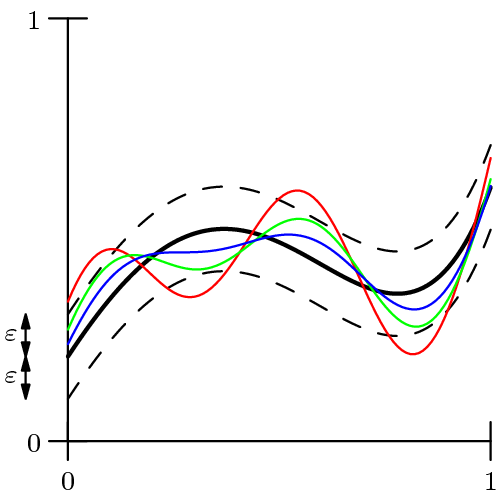
\includegraphics[width=0.4\textwidth]{pointwise}

            \subsubsection{Convergência Uniforme}

                Uma sequência de funções $u_n (x)$ converge uniformemente para $u(x)$ se para todo $x \in [a,b]$ e para todo $\epsilon >0$, existir $N=N(\epsilon)$ tal que $|u_n (x) - u(x)| < \epsilon$ sempre será atendido se $n>N$. Graficamente, temos a seguinte representação da convergência uniforme:

                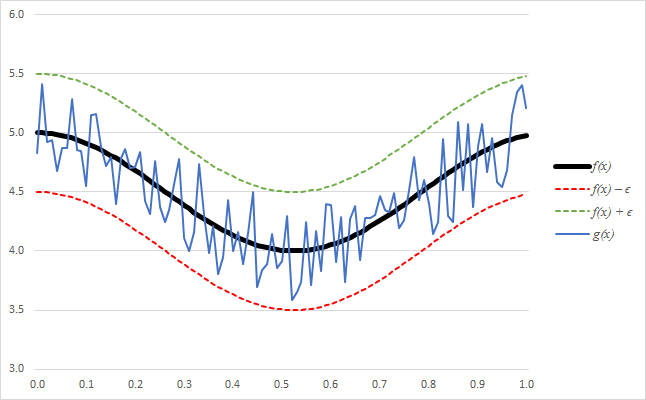
\includegraphics[width=0.4\textwidth]{uniform}


            \subsubsection{Convergência na Média Quadrática}

                Para as séries de Fourier, a convergência mais importante é a convergência na média quadrática. Se para todo
$\epsilon >0$ existir $N=N(\epsilon)$ tal que:

                $$\{\int_{a}^{b} |u_n (x) - u(x)|^2 dx\}^{\frac{1}{2}} < \epsilon$$

                Graficamente, a convergência em média quadrática pode ser observada na seguinte aproximação por série de Fourier:

                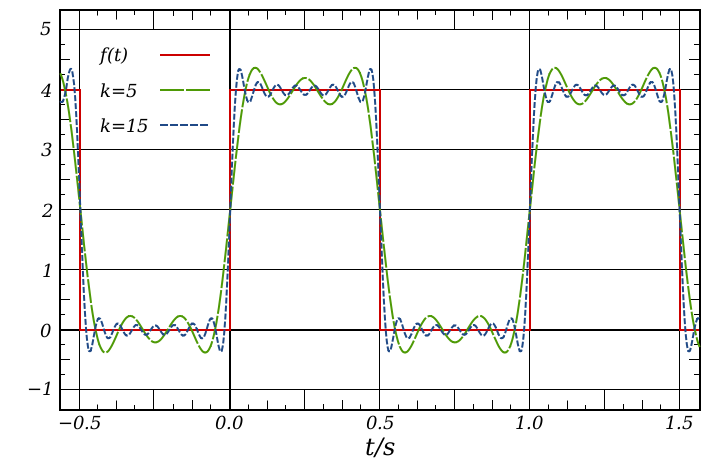
\includegraphics[width=0.4\textwidth]{conv_fourier}


                Nos pontos de descontinuidade observamos uma amplitude dos modos de Fourier que é maior que as amplitudes dos pontos de continuidade, esse fenômeno é conhecido pelo nome de Fenômeno de Gibbs. Além disso, notamos quem nas descontinuidades há uma convergência para o valor médio do salto. O teorema a seguir tratará desse resultado.
                

            \begin{theorem}	
                
                Teorema de Fourier: a série de Fourier de uma função contínua por partes e suficientemente suave converge ponto a ponto em toda a reta $ \mathbb{R} $. Se $ F(x) $ representar a extensão periódica de $ f(x) $, então no ponto $ x_{0} $ em que $ F(x) $ é contínua, a série converge para $ F(x_{0}) $; se $ x_{0} $ for um ponto de descontinuidade, a série converge para:

                $$  \frac{F(x_{0}^{+})+F(x_{0}^{-})}{2}.$$
            \end{theorem}

            \begin{example}	
                Extensão periódica da função degrau.
            \end{example}

    \section{Séries de Fourier de Senos e Cossenos}

        A depender da paridade da função, a série de Fourier de uma função pode ser representada apenas como uma série de senos ou cossenos. Relembrando: 

        \

        Se a função $f(x)$ é par:
        $$ \int_{-L}^{L} f(x)\ cos\left(\frac{k\pi x}{L}\right) dx = 2 \int_{0}^{L} f(x)\ cos\left(\frac{k\pi x}{L}\right)dx\ ,\ \mbox{ e } $$

        $$\int_{-L}^{L}f(x)\ sen\left(\frac{k\pi x}{L}\right) dx =0 \ ,\ \mbox{então }\ \ f(x) = \frac{a_{0}}{2} + \sum_{k=1}^{\infty}(a_{k} \  cos\left(\frac{k\pi x}{L}\right))  $$ 

        Se a função $f(x)$ é ímpar:
        $$ \int_{-L}^{L} f(x)\ cos\left(\frac{k\pi x}{L}\right) dx = 0 $$  e  $$ \int_{-L}^{L} f(x)\ sen\left(\frac{k\pi x}{L}\right) dx =2 \int_{0}^{L} f(x)\ sen\left(\frac{k\pi x}{L}\right)dx\ ,$$

        logo $$\ \ f(x) =  \sum_{k=1}^{\infty}(b_{k} \  sen\left(\frac{k\pi x}{L}\right)).    $$ \\ 

        Esses resultados implicam em:
        \begin{itemize}
            \item $ 1, cos(x), cos(2x), cos(3x), ... $ formam uma base para as funções contínuas por partes pares em $ [-\pi,\pi] $;
            \item $ sen(x), sen(2x), sen(3x), ... $ formam uma base para as funções contínuas por partes ímpares em $ [-\pi,\pi] $.
        \end{itemize}\


        Em muitas situações, deseja-se obter uma expansão em série de Fourier de uma função definida apenas no intervalo $ [0,\pi] $. Isso pode ser feito se utilizarmos o conceito de extensão periódica par ou ímpar, $ E_{f}(x) $ e $ O_{f}(x) $, respectivamente:

        $$ E_{f}(x)dx = \begin{cases}

        f(x), & 0 \leq x \leq \pi \\ 

        f(-x), & -\pi \leq x <0

        \end{cases}$$

        $$ O_{f}(x)dx = \begin{cases}

        f(x), & 0 \leq x \leq \pi \\

        -f(-x), & -\pi \leq x <0.

        \end{cases}$$

        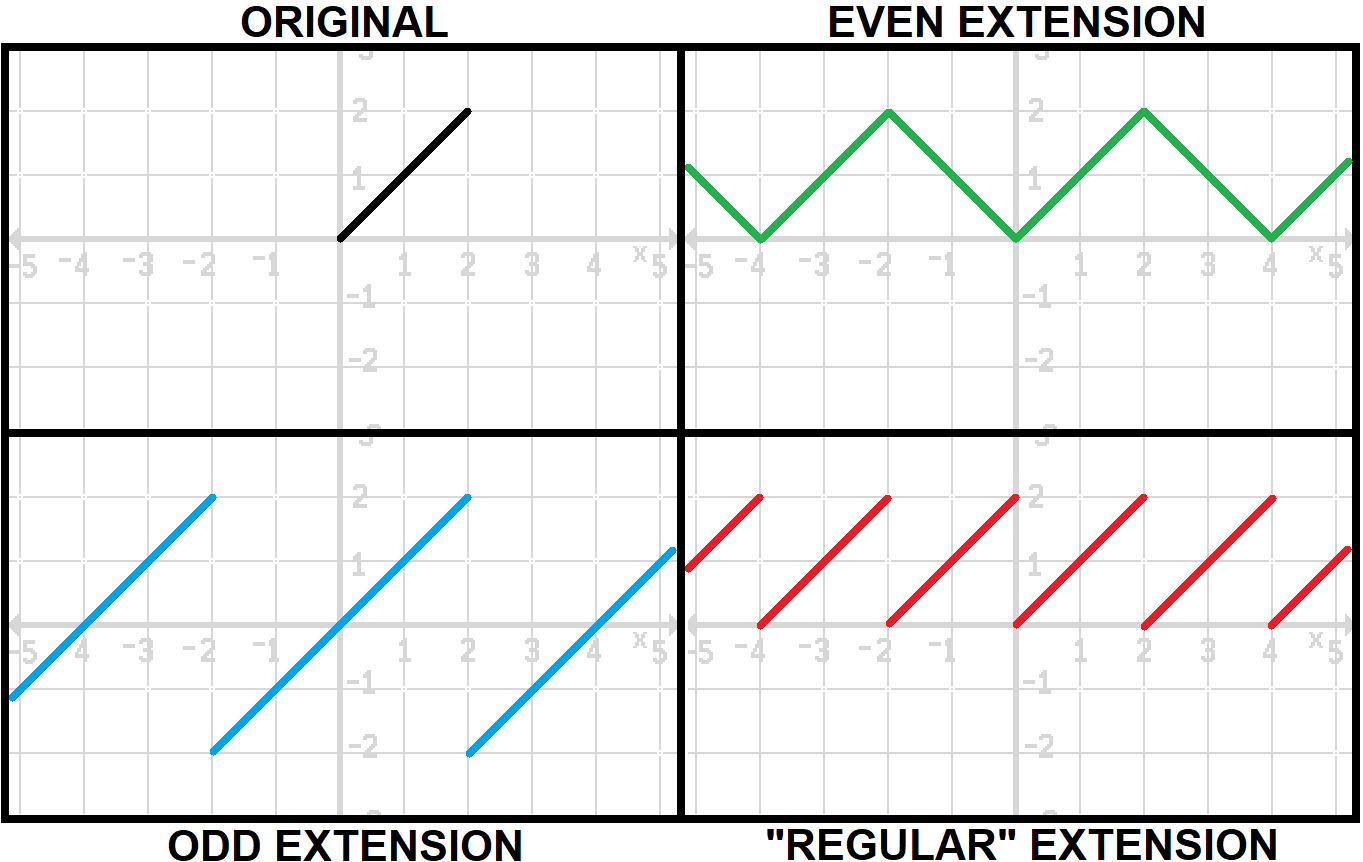
\includegraphics[width=0.4\textwidth]{even_odd}


        \begin{example}	
            Determinar a série de Fourier em cossenos e senos de $f(x) = x^2$ em $[0, \pi]$.
        \end{example}

    \section{Série de Fourier Complexa}

        \subsection{Fórmula de Euler}

            
            Série de Taylor para $ sen(x), cos(x), e^{x}: $ \

            $\displaystyle sen(x)=x-\frac{x^{3}}{3!}+\frac{x^{5}}{5!}-\frac{x^{7}}{7!}+... $ \\ 

            $\displaystyle cos(x)=1-\frac{x^{2}}{2!}+\frac{x^{4}}{4!}-\frac{x^{6}}{6!}+... $ \\ 

            $\displaystyle  e^{x}(x) = 1 + x+\frac{x^{2}}{2!}+\frac{x^{3}}{3!}+ \frac{x^{4}}{4!} + ... $ \\ 

            Faremos $ \displaystyle e^{ix}= 1 + (ix) + \frac{(ix)^{2}}{2!} + \frac{(ix)^{3}}{3!}+... $ , \\
            Notando que:\\ 
            $i^{1}=i \ \ \ \ \ \ \ \ i^{5}=i $\\
            $i^{2}=-1 \ \ \ \ \ i^{6}=-1$\\
            $i^{3}=-i \ \ \ \ \ i^{7}=-i$\\
            $i^{4}=+1 \ \ \ \ \ i^{8}=+1 $. \\ 

            Logo:
            $$  \displaystyle e^{ix}= 1 + ix - \frac{x^{2}}{2!} - \frac{ix^{3}}{3!} + \frac{x^{4}}{4!}+\frac{ix^{5}}{5!}+... \mbox{ e rearrumando,}  $$

            $$  \displaystyle e^{ix} = \left(1-\frac{x^{2}}{2!}+\frac{x^{4}}{4!}- \frac{x^{6}}{6!} + \frac{x^{8}}{8!}+...\right) + i \left(x-\frac{x^{3}}{3!}+ \frac{x^{5}}{5!}- \frac{x^{7}}{7!}+... \right) $$

            O primeiro termo entre parêntesis é a série de Taylor para a função $\cos{x}$, enquanto que o outro termo entre parêntesis é a série de Taylor para a função $\sin{x}$.

            $$ e^{ix} = cos(x) + i\ sen(x)   $$ \


        \subsection{Determinação da Série de Fourier Complexa}

        
            O conjunto $ 1, e^{ix}, e^{-ix}, e^{2ix}, e^{-2ix}, ... $ forma uma base contável para as funções contínuas por partes em $ [-\pi,\pi] $. Dessa forma, podemos escrever a série de Fourier complexa como:

            $$ f(x)=\sum_{k=-\infty}^{+\infty} c_{k}\ e^{ikx} $$ \

            $$ f(x) = \frac{a_{0}}{2} + \sum_{k=1}^{\infty} \left[ a_{k}\left( \frac{e^{ikx} + e^{-ikx}}{2}\right) + b_{k}\left( \frac{e^{ikx}-e^{-ikx}}{2i} \right) \right] $$ \

            $$ f(x) = \frac{a_{0}}{2} + \sum_{k=1}^{\infty} \left[ \frac{(a_{k}-ib_{k})}{2} e^{ikx} \right] + \sum_{k=1}^{\infty} \left[ \frac{(a_{k}+ib_{k})}{2} e^{-ikx} \right]  $$ \

            $$ f(x) = \sum_{k=-\infty}^{k=\infty} c_{k}\ e^{ikx}  \, \ \ \mbox{  onde:}$$ 


            $$ c_{k}= \begin{cases}

                \displaystyle \frac{a_{0}}{2}, &  k=0 \\ \\

                \displaystyle \frac{(a_{k}-ib_{k})}{2}, & k=1,2,3,... \\ \\

                \displaystyle \frac{(a_{-k}+ib_{-k})}{2}, & k=-1,-2,-3,...

            \end{cases}   $$ 

            Para $ k>0 $, temos:
            $$ c_{k}=\frac{1}{2} (a_{k}-ib_{k}) = \frac{1}{2\pi} \int_{-\pi}^{\pi} \left(cos(kx) - i\ sen(kx) \right)f(x)dx $$

            $$=  \frac{1}{2\pi} \int_{-\pi}^{\pi} f(x) e^{-ikx} dx $$ \\

            Para $ k<0 $, temos:
            $$ c_{k}=\frac{1}{2} (a_{-k}+ib_{-k}) = \frac{1}{2\pi} \int_{-\pi}^{\pi} \left(cos(-kx) + i\ sen(-kx) \right)f(x)dx$$
            $$=  \frac{1}{2\pi} \int_{-\pi}^{\pi} f(x) e^{-ikx} dx $$ \

            \begin{example}	
                Obter a série de Fourier complexa para $f(x) = \sin(x)$ em $[-\pi, \pi]$.
            \end{example}

            \begin{example}	
                Série de Fourier complexa de $$ f(x) = \begin{cases} 1, \;0<x<a (a<\pi) \\  0, \text{  em todo o resto} \\ \end{cases}$$ 
            \end{example}

            \begin{example}	
                $f(x) = x^2$ no intervalo $[-1,1]$.
            \end{example}

            \begin{example}	
                Série de Fourier complexa de $$ f(x) = \begin{cases} \sin(x), \;0<x<\pi  \\  0, \pi < x< 2\pi \\ \end{cases}.$$ 
            \end{example}

            \begin{example}	
                Converter a série do exemplo 6.2 para a forma real.
            \end{example}

            \begin{example}	
                Converter para a forma complexa a série de Fourier real da função degrau (exemplo 4.2).
            \end{example}

    \section{A Identidade de Parseval (Uma nova visão)}


        O Teorema 1.5 (seção 1.2) estabelece a identidade de Parseval: $ \displaystyle \sum_{i=1}^{\infty} (x,e_{i})^{2} = ||x||^{2} $. Para uma função periódica de período $ 2L $ e sejam $ c_{k} (k=0,\pm1, \pm2, ...) $, os coeficientes complexos da função $f(x)$, então:

        $$ \frac{1}{2L} \int_{-L}^{L} f^{2}(x)dx = \sum_{k=-\infty}^{\infty} |c_{k}|^{2}  $$ \

        Prova:

        Assumindo $\displaystyle f(x)= \sum_{k=-\infty}^{\infty} c_{k} e^{\frac{k\pi ix}{L}}\ $ e  $\ \displaystyle c_{k}=\frac{1}{2L}\int_{-L}^{L} f(x)e^{\frac{-k\pi ix}{L}} dx\ $, 

        temos $ f^{2}(x)=f(x)f(x) $, logo $\displaystyle f^{2}(x)=f(x) \sum_{k=-\infty}^{\infty} c_{k} e^{\frac{k\pi ix}{L}} = \sum_{k=-\infty}^{\infty} c_{k} f(x) e^{\frac{k\pi ix}{L}} $.

        \vspace{1cm}
        Integrando os 2 lados:
        \vspace{0.3cm}

        $\displaystyle \frac{1}{2L}\int_{-L}^{L} f^{2}(x)dx = \frac{1}{2L}\int_{-L}^{L}\sum_{k=-\infty}^{\infty} c_{k} f(x) e^{\frac{k\pi ix}{L}}dx = \frac{1}{2L} \sum_{k=-\infty}^{\infty} c_{k} \int_{-L}^{L} f(x) e^{\frac{k\pi ix}{L}}dx = \sum_{k=-\infty}^{\infty} c_{k}\bar{c_{k}} = \sum_{k=-\infty}^{\infty} |c_{k}|^{2} $ \\ \\

        A versão real da mesma Identidade é:


        $$ \frac{1}{L}\int_{-L}^{L} |f(x)|^{2} = \frac{1}{2} a_{0}^{2}  + \sum_{k=1}^{\infty} (a_{k}^{2} + b_{k}^{2}) $$ \

        \begin{example}	
            Utilizar a identidade de Parseval para a série de Fourier real de $f(x) = |x|$ em $[-\pi,\pi]$.
        \end{example}

        \begin{example}	
            Aplicar a identidade de Parseval na série de Fourier de $f(x) = 1+x$ em $[-\pi,\pi]$.
        \end{example}

    \section{Transformada de Fourier}

    Vimos que a série de Fourier permite que possamos representar funções periódicas como uma soma de cossenos e senos. Para funções nâo-periódicas a extensão desse conceito é a transformada de Fourier.  A transformada de uma função $f(t)$ é dada por:

    \begin{equation}	
        \mathcal{F}(\omega) = \mathbf{F}(f(t)) = \int_{-\infty}^{\infty} f(t)e^{-i\omega t} dt
    \end{equation}

    A transformada de Fourier inversa é:

    \begin{equation}	
        f(t)= \mathbf{F}^{-1}(\mathcal{F}(\omega)) = \frac{1}{2\pi} \int_{-\infty}^{\infty} \mathcal{F}(\omega)e^{i\omega t} dt
    \end{equation}

    A transformada de Fourier tem diversas propriedades, as principais são:

    \begin{description}
        \item[(i)] Linearidade - Se $f(t) = \alpha f_1(t) + \beta f_2(t)$, então:

        \begin{equation*}	
            \mathcal{F}(\omega) = \int_{-\infty}^{\infty} (\alpha f_1(t) + \beta f_2(t))e^{-i\omega t} dt= \alpha \mathcal{F}_1(\omega) + \beta \mathcal{F}_2(\omega)
        \end{equation}
        
    \item[(ii)] Escala de tempo - Se $f(t) = g(\alpha t)$, então: $$\mathcal{F}(\omega) = \frac{1}{|\alpha|}\mathcal{G}(\frac{\omega}{\alpha}).$$

        \item[(iii)] Deslocamento no tempo - Para $f(t) = g(t-a)$, então: $$\mathcal{F}(\omega) = \mathcal{G}(\omega)e^{-i\omega a}.$$

        \item[(iv)] Transformada da derivada - Se $f(t) = \frac{d^n}{dt^n}g(t)$, a transformada fica: $$\mathcal{F}(\omega) = (i\omega)^n \mathcal{G}(\omega).$$

        \item[(v)] Convolução - A transformada inversa do produto de duas funções $\matcal{F}(\omega)$ $\mathcal{G}(\omega)$ não é o produto de suas inversas. Em vez disso, temos uma operação binária chamada de convolução: 

            $$f(t) * g(t) = \int_{-\infty}^{\infty} f(\tau)g(t - \tau) d\tau.$$

            A transformada de Fourier da convolução é igual ao produto das das transformadas:

            $$ \mathbf{F}(f(t) * g(t)) = \mathbf{F}(f(t))\mathbf{F}(g(t)) = \mathcal{F}(\omega)\mathcal{G}(\omega).$$

    \end{description}

    \begin{example}	
        Vamos analisar a equação do movimento harmônico forçado com amortecimento:
        
        $$\frac{d^2}{dt^2}x(t) + 2\zeta \frac{d}{dt}x(t) + \omega_o^{2}x(t)= f(t).$$


    \end{example}

\end{multicols*}

\end{document}
